\section{Introduction}
\begin{frame}{Introduction}
  \begin{center}
    \begin{overlayarea}{\textwidth}{175px}

      \only<1>{
\includegraphics[height=200px]{brainstorming-1.pdf}}
      % Le but de cette conférence, c’est vous aider à bien commencer votre
      % projet. Ben oui, mais c’est quoi ce projet ?
      \only<2>{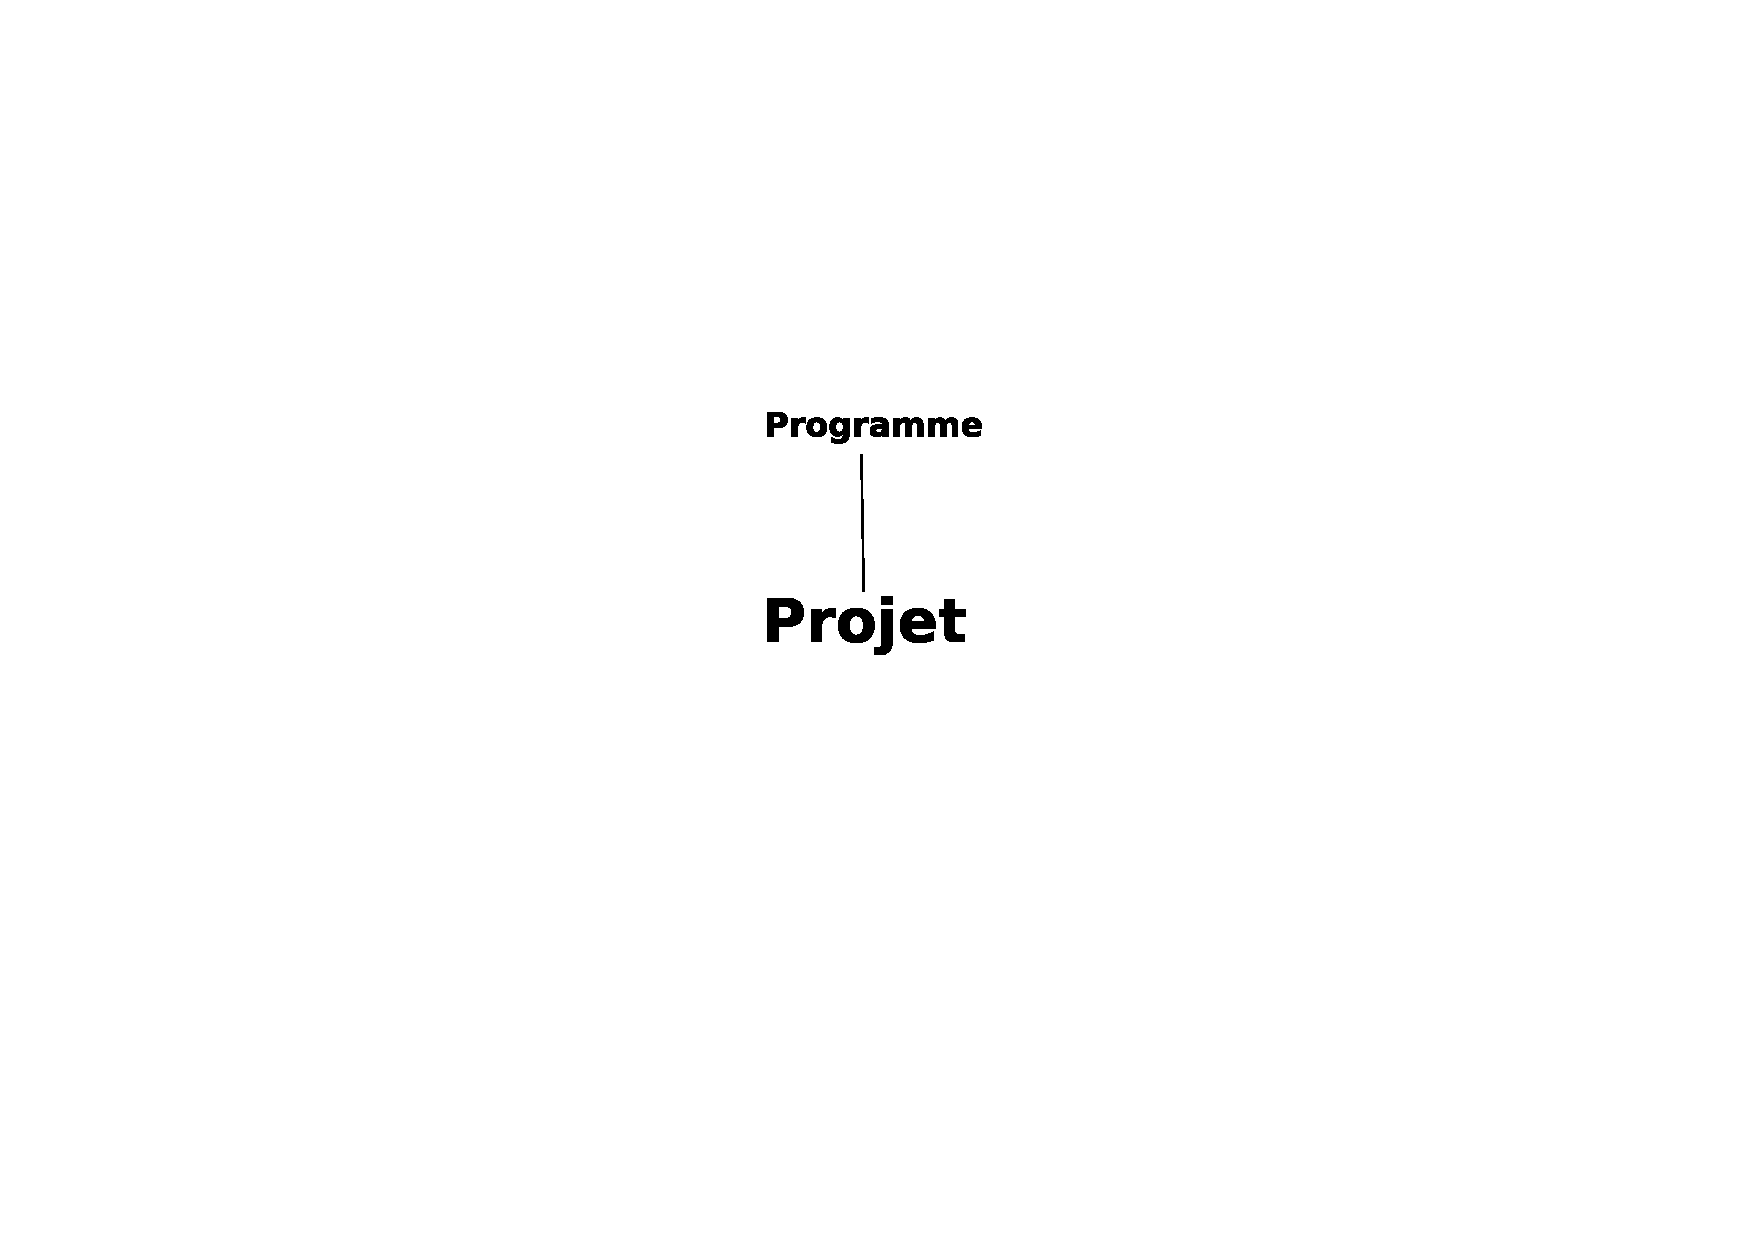
\includegraphics[height=200px]{brainstorming-2.pdf}}
      % Votre projet, c’est de concevoir un programme. Ah, c’est un peu plus
      % précis.
      \only<3>{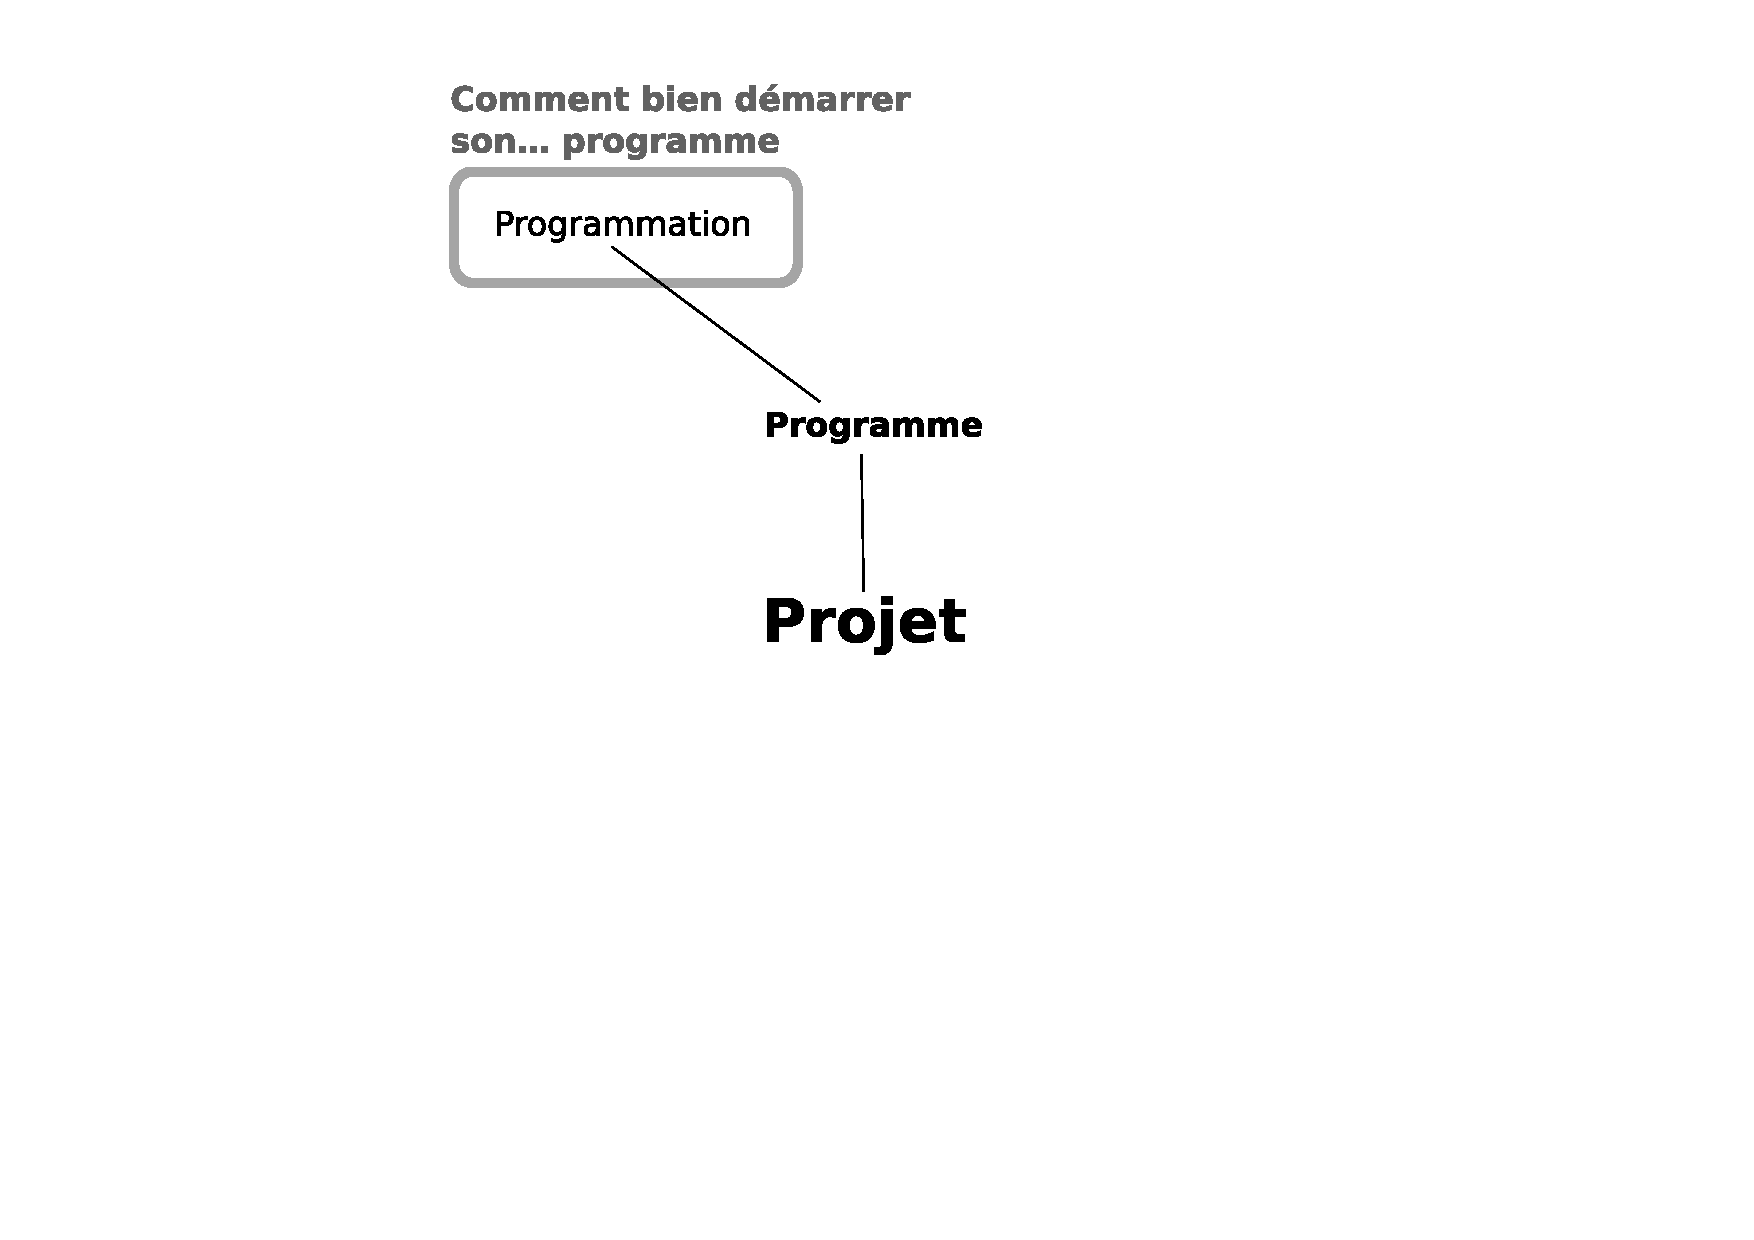
\includegraphics[height=200px]{brainstorming-3.pdf}}
      % Du coup, il va falloir que vous programmiez un peu. Logique. C’est le
      % premier volet de cette conférence : comment allez-vous vous y prendre ?
      \only<4>{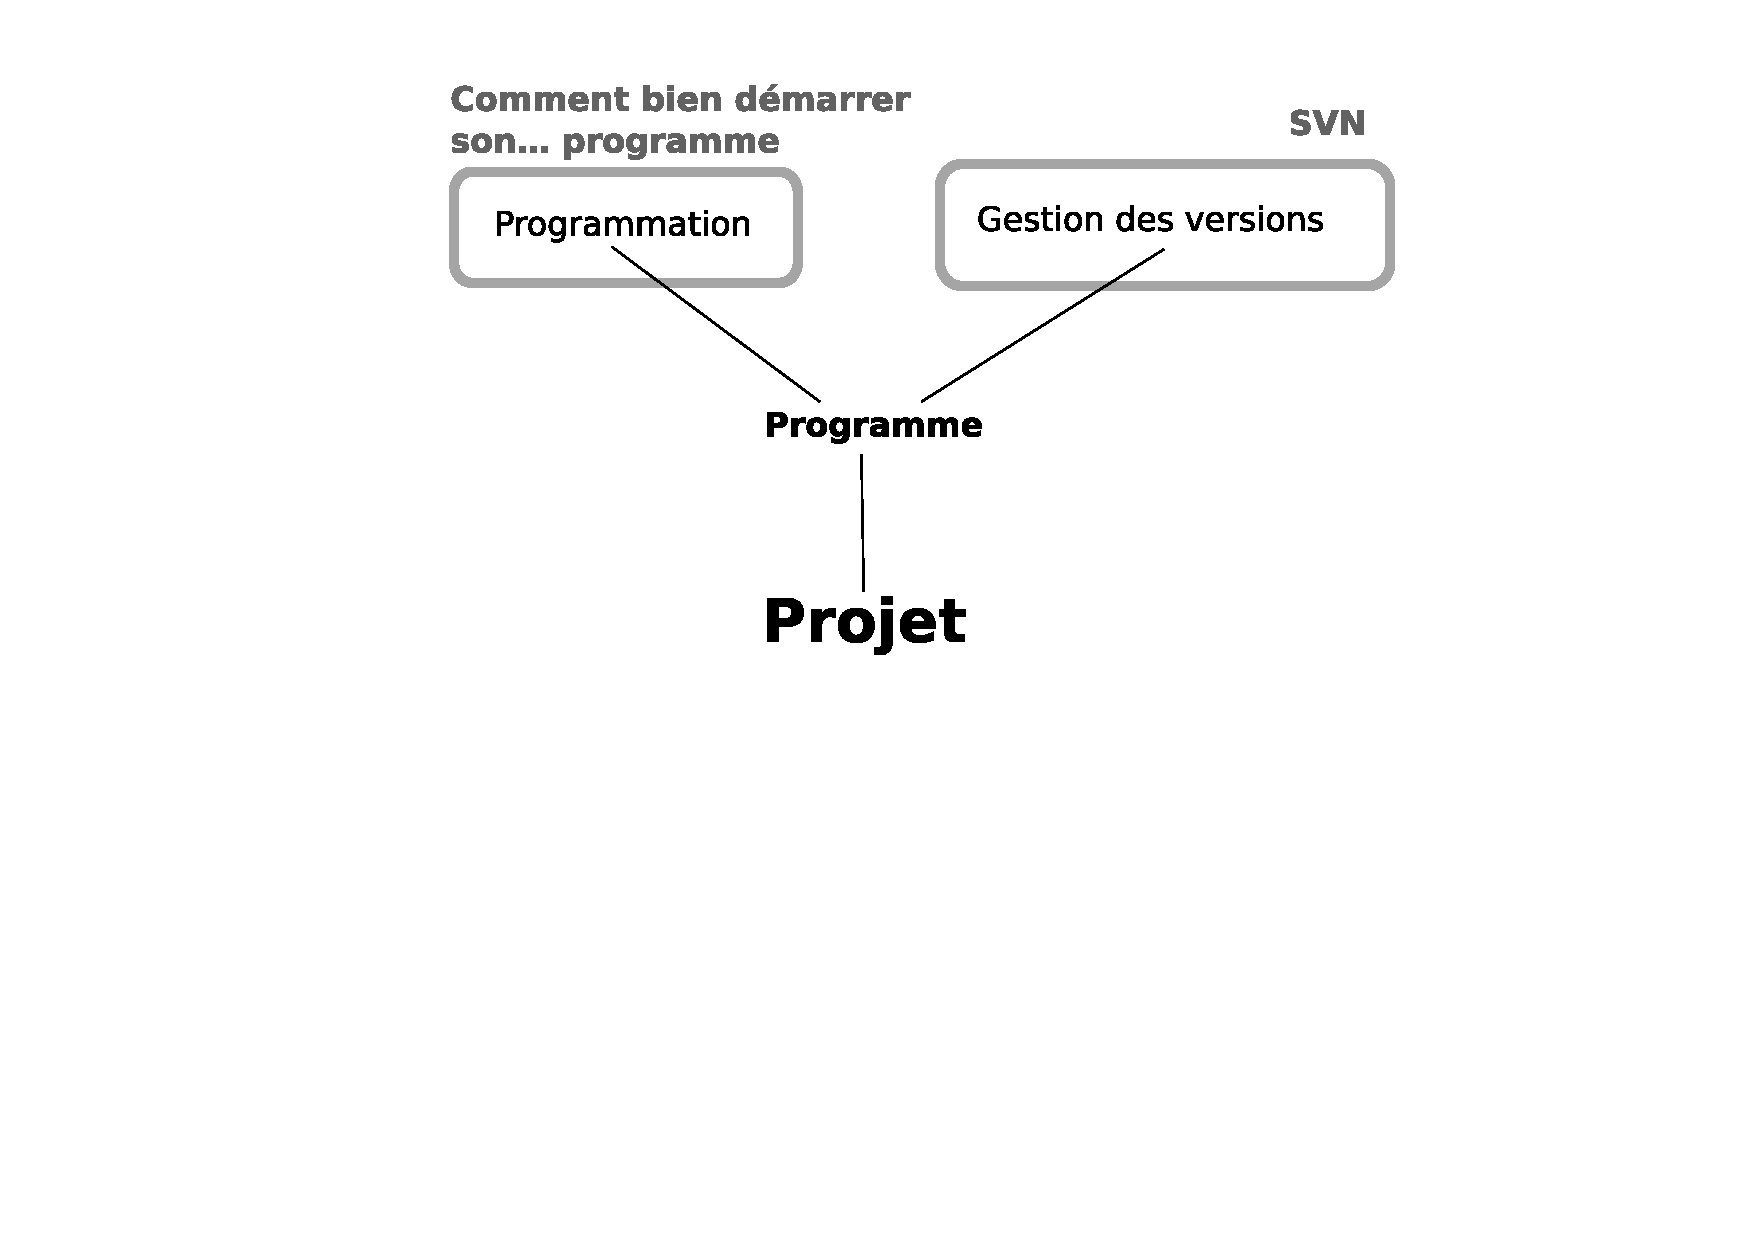
\includegraphics[height=200px]{brainstorming-4.pdf}}
      % Le code, c’est bien, mais… il faut maîtriser son évolution ! SVN, Git,
      % Mercucial et d’autres sont là pour vous faciliter la tâche. La deuxième
      % partie de cette conférence porte sur le principe et l’utilisation de SVN.
      \only<5>{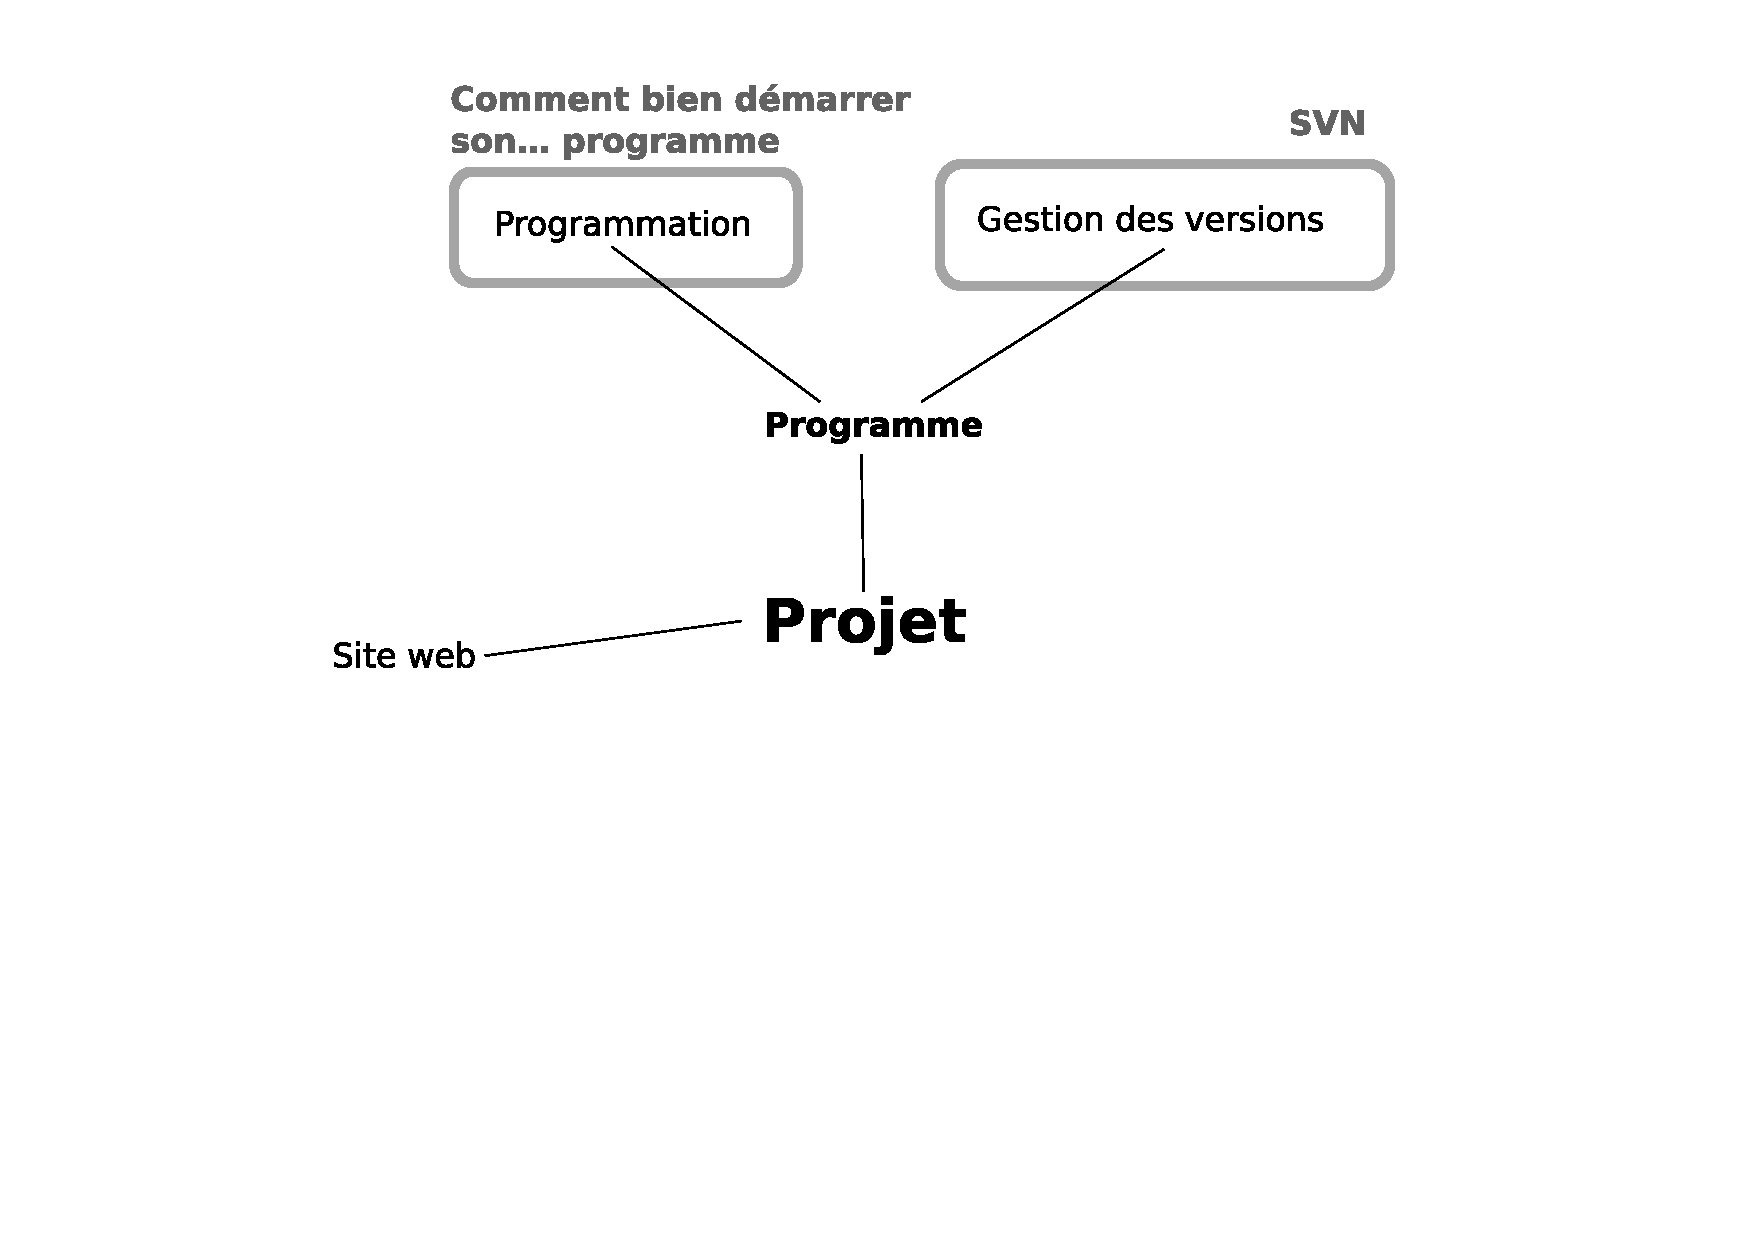
\includegraphics[height=200px]{brainstorming-5.pdf}}
      % Bon, le projet exige que vous concoctiez aussi un site web, une vitrine
      % de votre projet. Le site est assez important, comme toute la
      % communication autour de votre projet, mais ça reste simple et facile à
      % faire… Débrouillez-vous ! :-)
      \only<6>{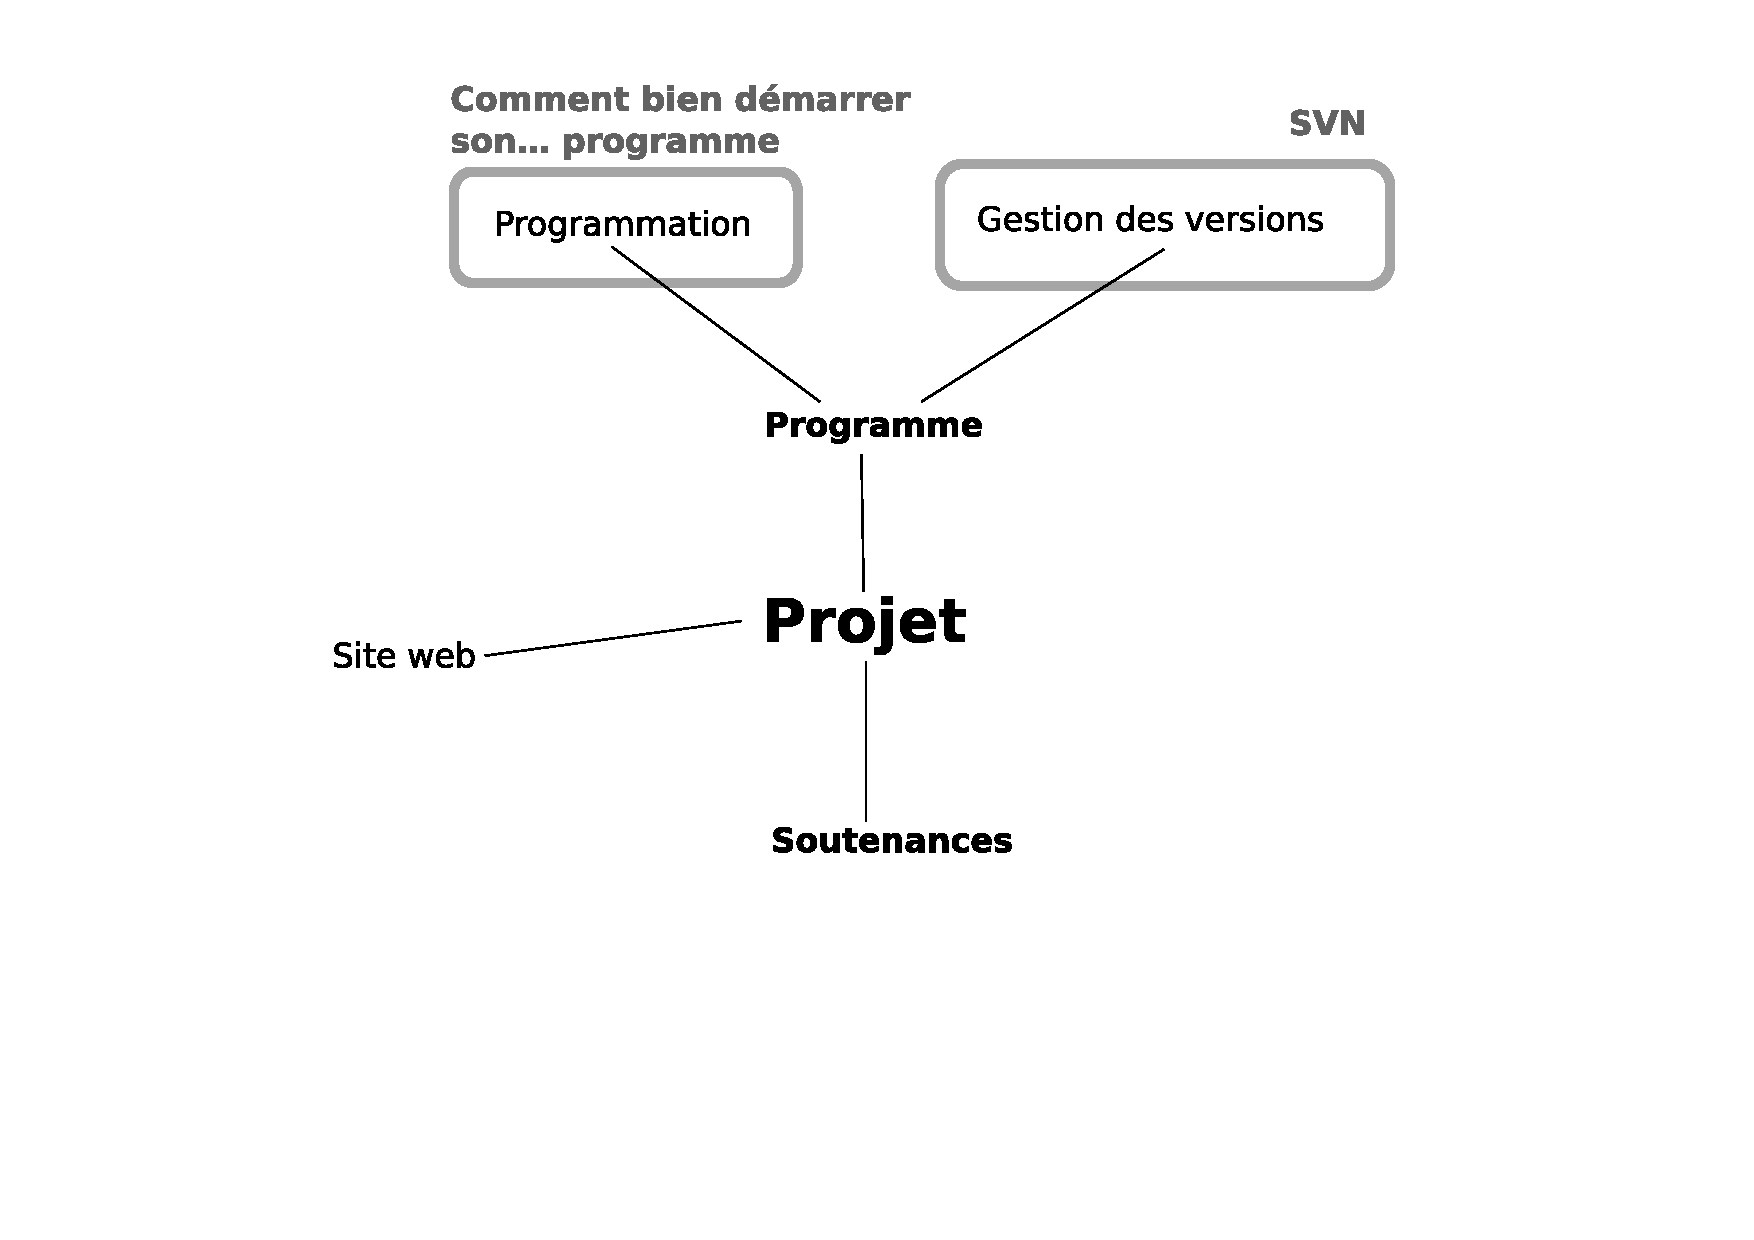
\includegraphics[height=200px]{brainstorming-6.pdf}}
      % Krisboul vous donne du travail et veut vous observer pour être certain
      % que vous bossez ! C’est pour cela que 4 soutenances sont prévues tout au
      % long de l’année.
      \only<7>{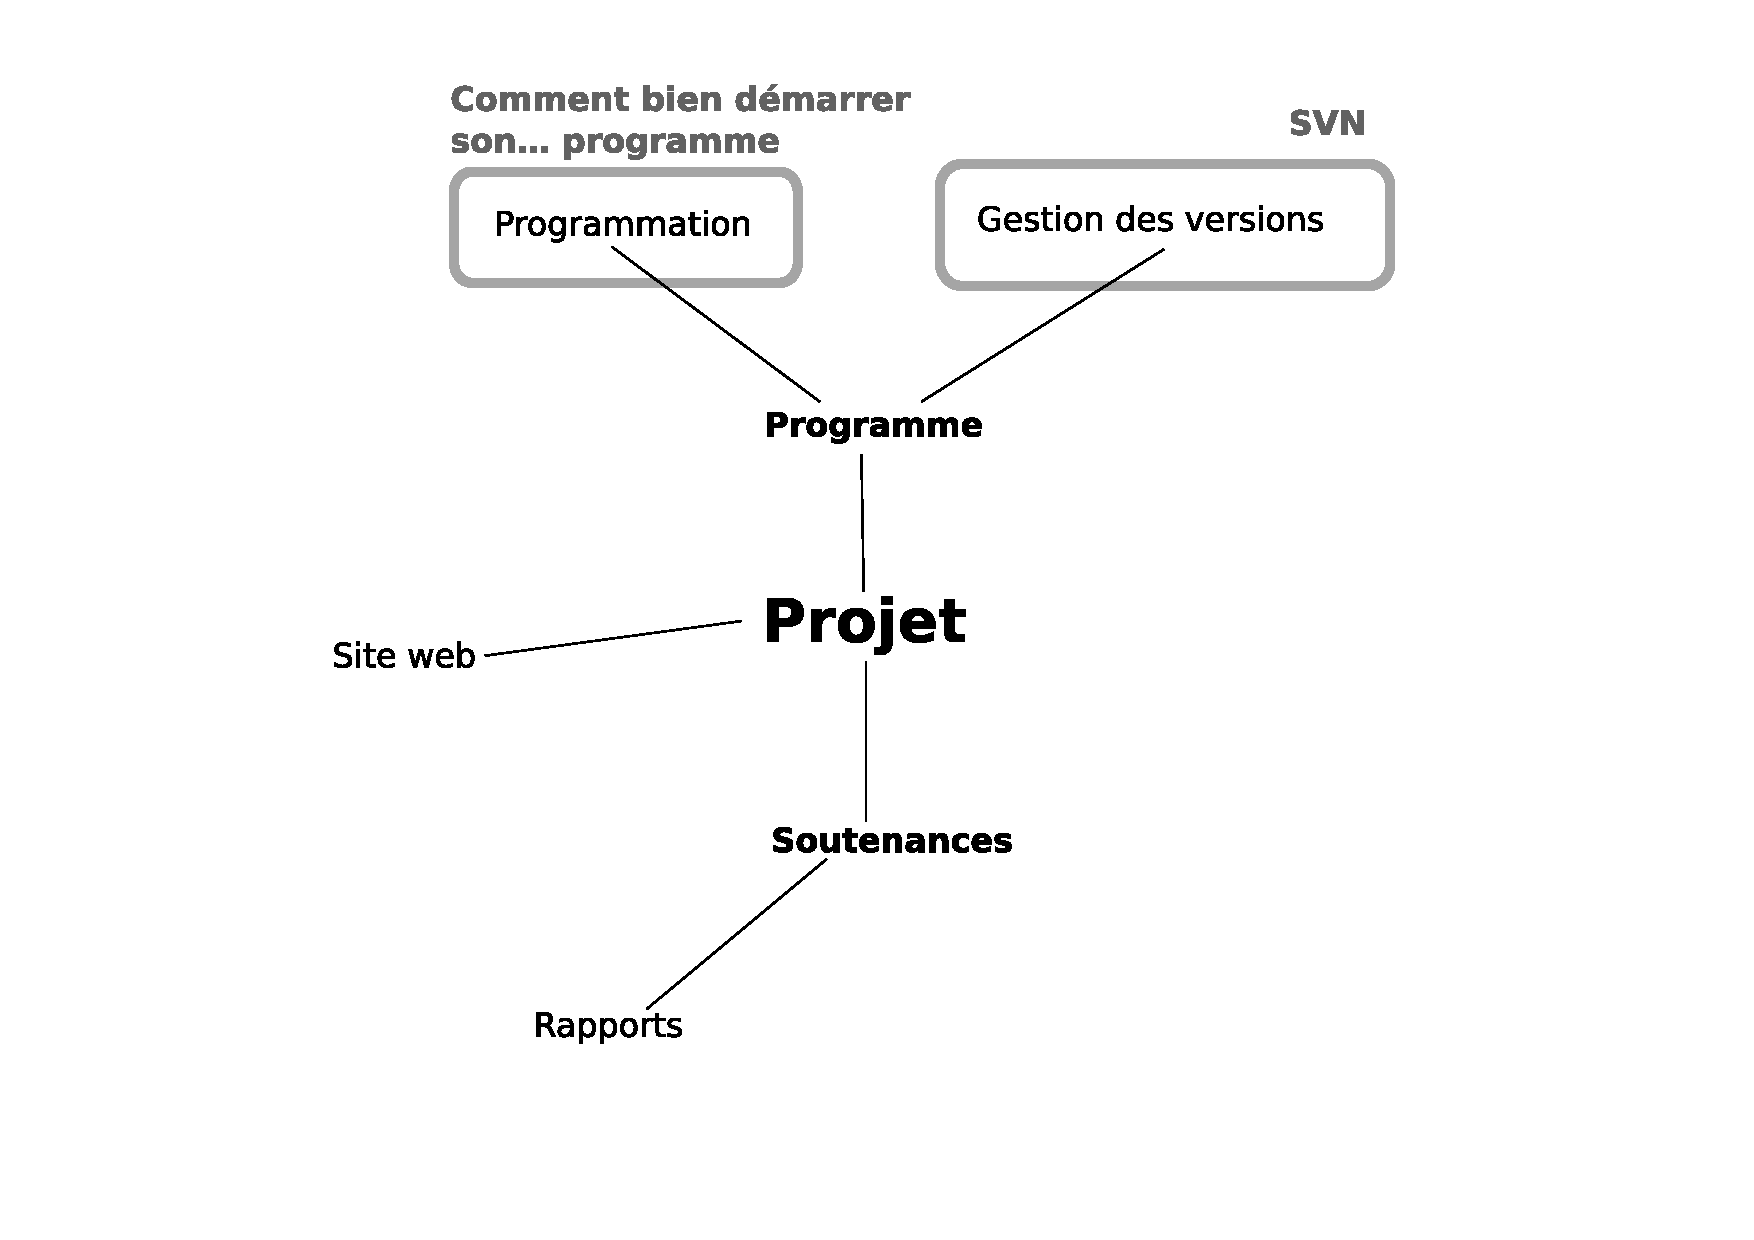
\includegraphics[height=200px]{brainstorming-7.pdf}}
      % À chaque soutenance, vous avez un rapport à fournir…
      \only<8>{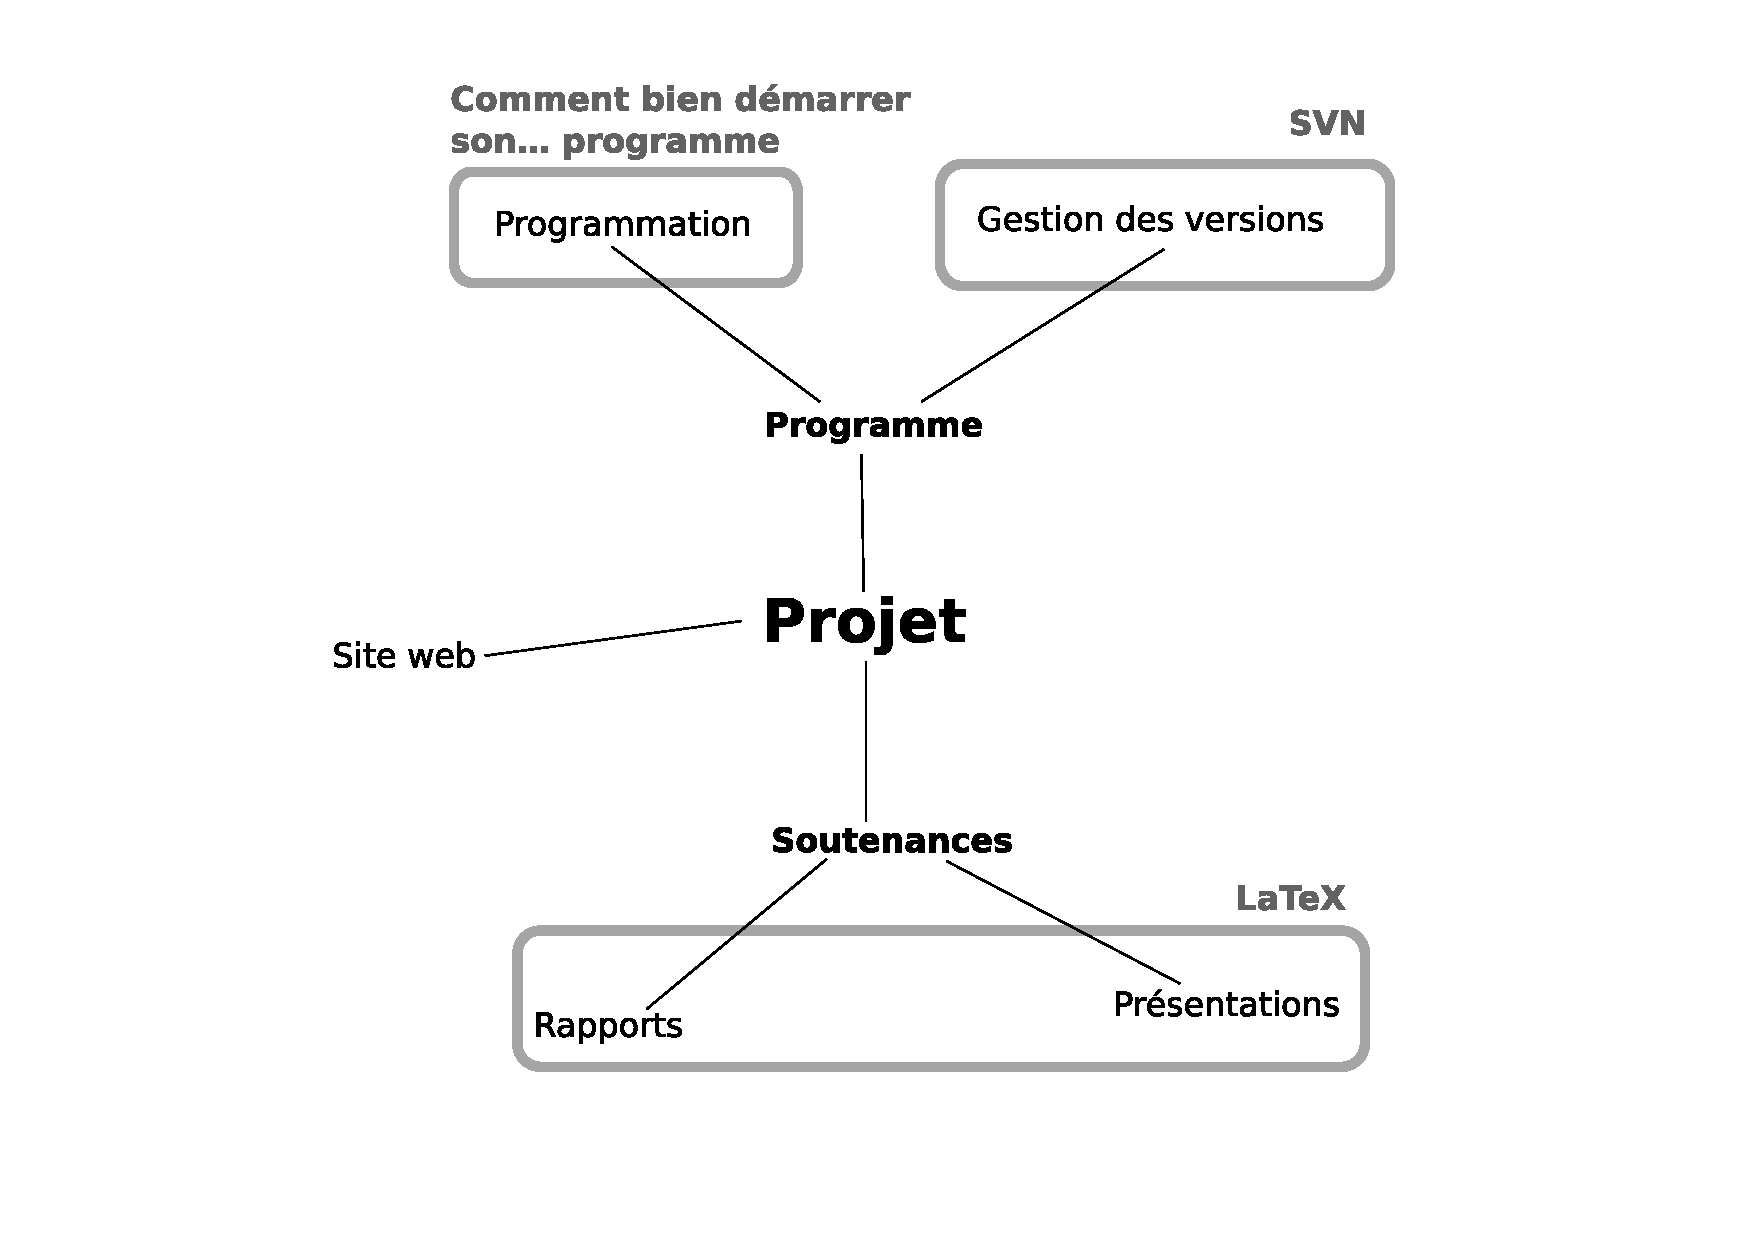
\includegraphics[height=200px]{brainstorming-8.pdf}}
      % … ainsi qu’une présentation à faire. Le contenu n’est pas l’objet de la
      % conférence (c’est dans le sujet, le reste n’est que quelques conseils
      % qu’on peut vous donner), en revanche nous vous conseillons d’utiliser
      % LaTeX pour mettre en forme vos rapports et vos diaporamas.
      \only<9>{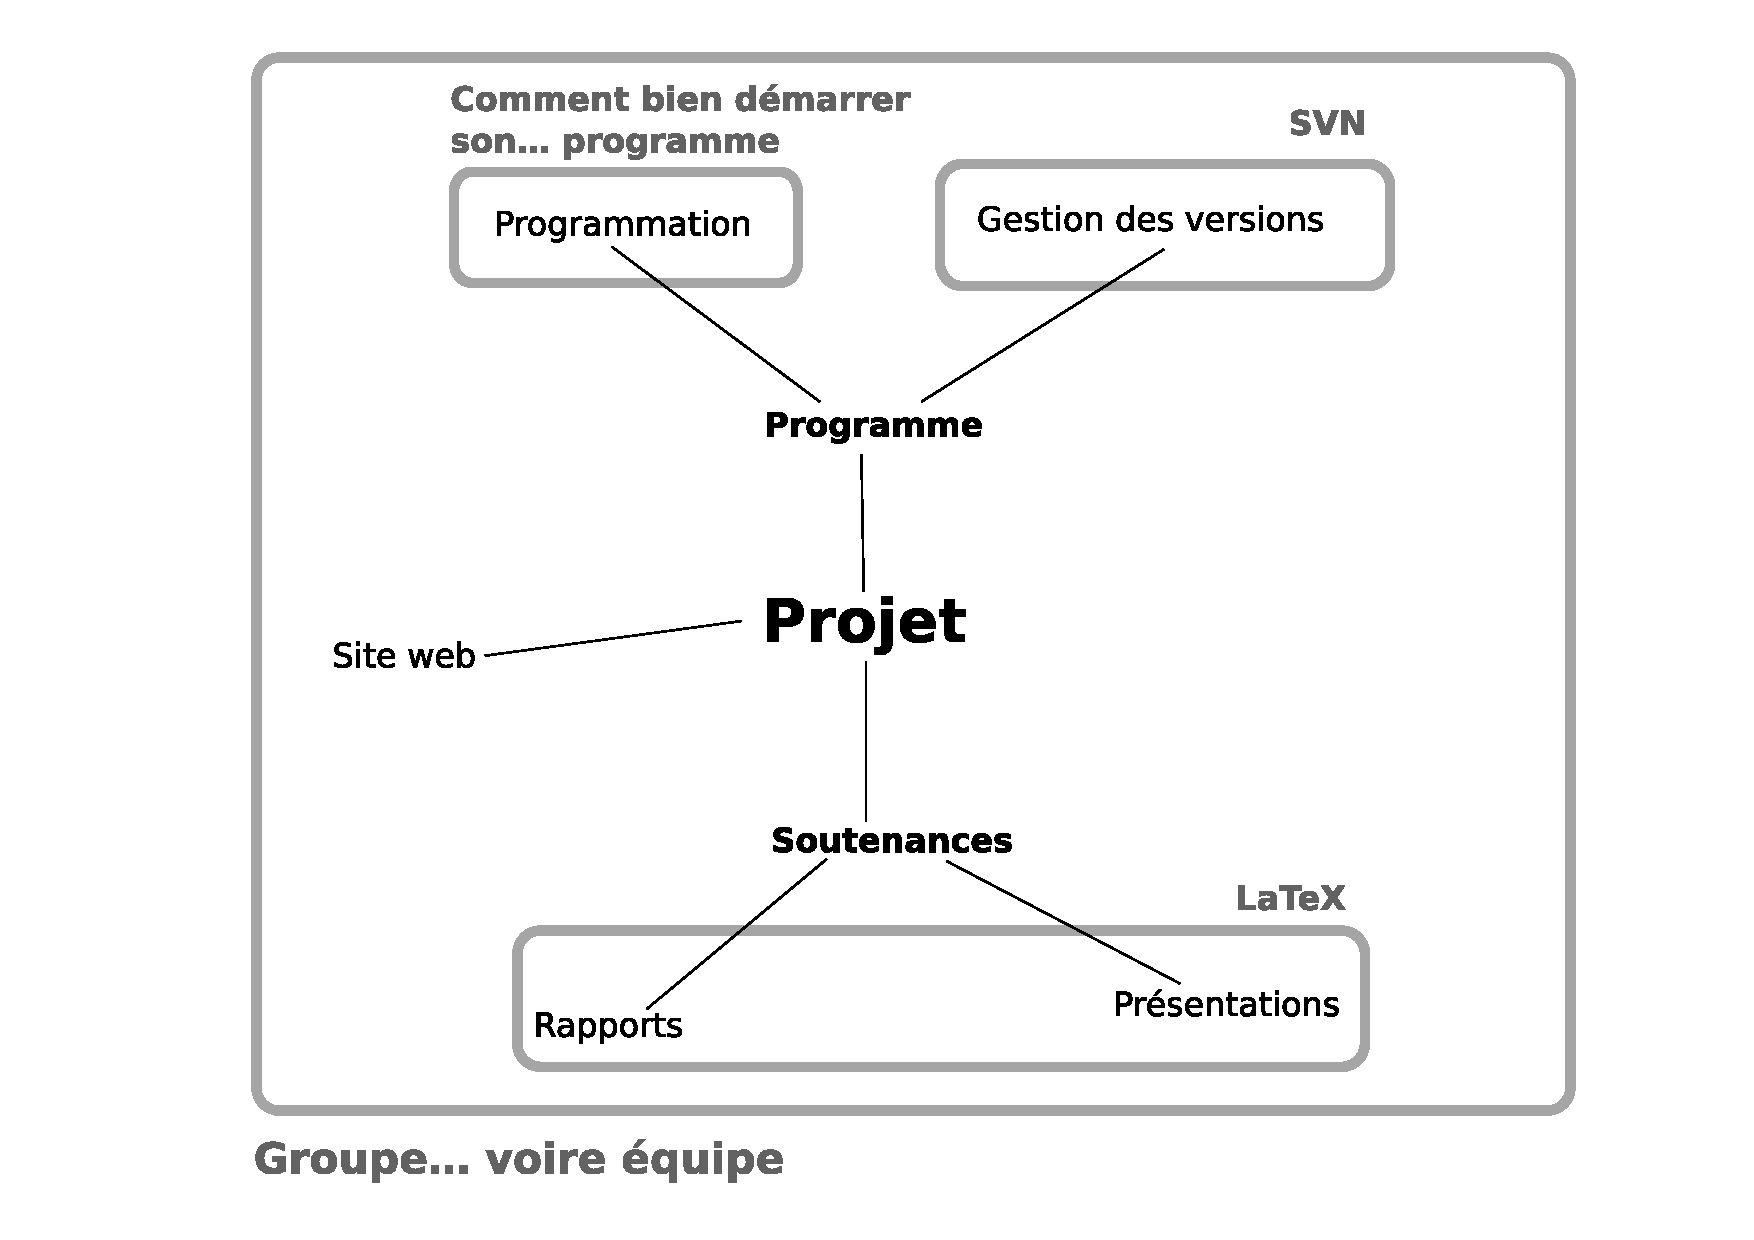
\includegraphics[height=200px]{brainstorming-9.pdf}}
      % Tout ce qui touche à votre projet est à faire en équipe. La gestion de
      % l’équipe est extrêmement importante ! … mais ce n’est pas ici qu’on va
      % vous expliquer comment vous y prendre.

    \end{overlayarea}
  \end{center}
\end{frame}
